\documentclass{beamer}
\usepackage[ngerman]{babel}
\usepackage[utf8]{inputenc}
\usepackage[T1]{fontenc}
\usepackage{lmodern}

% bibliography
\usepackage{natbib}

% theme and colortheme
\usetheme{Berkeley}
\usecolortheme{spruce}
\setbeamertemplate{caption}[numbered]

% footer setting
\beamertemplatenavigationsymbolsempty
\setbeamertemplate{footline}[frame number]

% math mode settings
\usepackage{mathtools}
\usepackage{amssymb}
\usepackage{euler}
\usepackage[makeroom]{cancel}
\renewcommand{\deg}{\ensuremath{^{\circ}}}
\renewcommand{\epsilon}{\varepsilon}

% Grafikumgebungen
\usepackage{graphicx}
\usepackage{subcaption}
%\captionsetup[subfigure]{labelformat=parens, labelsep=quad}
\usepackage{floatflt}
\usepackage{float}

% table of contents at beginning of each section
%\AtBeginSection[]
%{
%  \begin{frame}
%    \frametitle{Contents}
%    \tableofcontents[currentsection]
%  \end{frame}
%}

% information to be included in the title page
\title{Bestimmung der Wolkenhöhe mittels Pyrgeometer}
\author{Lehrexkursion 2016 - Wolkenfernerkundung}
\date{\today}

%%%%%%%%%%%%%%%%%%%%%%%%%%%%%%%%%%%%%%%%%%%%%%%%%%
\begin{document}
\begin{frame}
\titlepage
\end{frame}

\section{Hintergrund}
\begin{frame}{Hintergrund}
\begin{columns}
\begin{column}{0.6\textwidth}
\begin{itemize}
  \vfill\item Bewölkung erhöht die langwellige Einstrahlung
  \vfill\item Die Strahlungsintensität hängt von der Temperatur des emittierenden Körpers ab \[ I \propto T\]
  \vfill\item Strahlungsmessungen enthalten Informationen über die Wolkentemperatur
              und ermöglichen so Rückschlüsse auf die Wolkenhöhe
  \vfill
\end{itemize}
\end{column}

\begin{column}{0.4\textwidth}
\begin{figure}[ht]
    \centering
    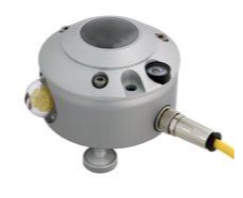
\includegraphics[width=1\textwidth]{figures/pyrgeometer.png}
    \caption{Pyrgeometer}
    \label{fig:pyrgeometer}
\end{figure}
\end{column}
\end{columns}
\end{frame}

\section{Pyrgeometer}
\begin{frame}{Pyrgeometer}
\begin{columns}
\begin{column}{0.6\textwidth}
\begin{itemize}
  \vfill\item Messung der atmosphärischen Gegenstrahlung $L\downarrow$\\
              (5 bis 50\,$\mu$m)
  \vfill\item Schwarze Sensoroberfläche mit Abschirmung der kurzwelligen Einstrahlung
  \vfill\item Langwellige Nettostrahlung wird durch Wärmeleitung in einer Thermosäule ausgeglichen
\vfill
\end{itemize}
\end{column}

\begin{column}{0.4\textwidth}
\begin{figure}[ht]
    \centering
    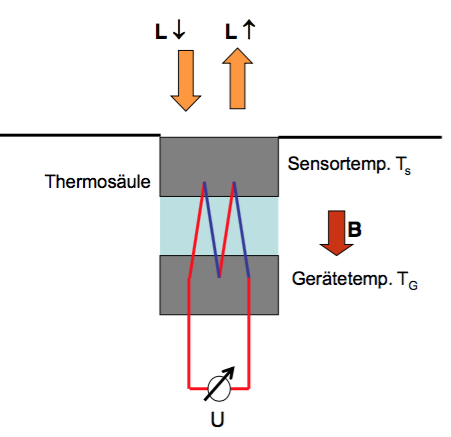
\includegraphics[width=1\textwidth]{figures/pyrgeometer_funktion.png}
    \caption{Aufbau}
    \label{fig:pyrgeometer_funktion}
\end{figure}
\end{column}
\end{columns}

\begin{alertblock}{Pyrgeometerformel}
  \centering$ L\downarrow = \lambda (T_S - T_G) + \sigma T_G^4 \approx cU + \sigma T_G^4 $
\end{alertblock}
\end{frame}

\section{Konzept}
\begin{frame}{Konzept}
\begin{itemize}
  \vfill\item Berechnung der Wolkentemperatur aus den Strahlungsmessungen des Pyrgeometers
    \begin{itemize}
      \item Stefan-Boltzmann-Gesetz $E = \sigma T^4$
      \item Eventuelle Berücksichtigung des Bedeckungsgrades
    \end{itemize}
  \vfill\item Zuordnung der Wolkentemperatur zu einer Höhe
  \begin{itemize}
    \item adiabatische Abnahme der Temperatur ausgehend\\
          von der Bodentemperatur $T_s$
    \item Standardatmosphäre mit angepasster $T_s$
    \item Radiosondenaufstieg
  \end{itemize}
  \vfill
\end{itemize}
\end{frame}

\end{document}
